\documentclass[12pt,a4paper]{article}

\usepackage[utf8]{inputenc}
\usepackage[T1]{fontenc}
\usepackage{mathpazo}
\usepackage[margin=2.5cm]{geometry}
\usepackage{setspace}
\doublespacing
\usepackage{graphicx}
\usepackage{booktabs}
\usepackage{multirow}
\usepackage{natbib}
\usepackage{url}
\usepackage{hyperref}
\hypersetup{colorlinks=true,linkcolor=blue,citecolor=blue,urlcolor=blue}

\title{\textbf{Did Kelud Eruptions Accelerate Majapahit's Decline?\\An Exploratory Analysis of the Pararaton Chronicle}}

\author{Mukhlis Amien\textsuperscript{1*}}

\date{}

\begin{document}

\maketitle

\noindent\textsuperscript{1}Lab Data Sains, Universitas Bhinneka Nusantara, Malang, Indonesia\\
\noindent\textsuperscript{*}Corresponding author: amien@ubhinus.ac.id

\begin{abstract}
The \textit{Kitab Pararaton}, the primary chronicle of the Majapahit kingdom of East Java, ends not with a political event but with a volcanic eruption: \textit{guntur pawatugunung} (1481~CE).
We cross-reference 18 dated Pararaton political crises against the Global Volcanism Program (GVP) database for Gunung Kelud, the dominant stratovolcano of the Majapahit heartland.
Three lines of evidence converge: (1)~a permutation test shows crises cluster closer to preceding eruptions than expected by chance ($p = 0.037$, uncorrected; does not survive Bonferroni correction for multiple comparisons); (2)~the Kelud eruption rate during Majapahit's decline (1376--1527) was 2.18 times higher than during its peak; and (3)~all three geological events recorded in the Pararaton match the GVP database independently.
While no individual statistical test provides definitive evidence after correction for multiple comparisons, the convergence of temporal, rate-based, and textual evidence warrants further investigation.
We propose that Kelud eruptions destabilised the agricultural surplus sustaining the mandala system, and that the Pararaton author's editorial decision to close the chronicle with an eruption may encode causal awareness.

\medskip\noindent\textbf{Keywords:} Majapahit; Pararaton; Kelud; volcanic eruption; mandala theory; East Java
\end{abstract}

\section{Introduction}

Standard historiography attributes Majapahit's fall to succession disputes, the rise of Islamic coastal polities, and shifts in Chinese trade policy \citep{ricklefs2001,reid1993}.
All three factors are real, but none explain timing: succession disputes were endemic to pre-modern mandala polities; Islam predated the decline by centuries; Chinese trade shifts affected all maritime states equally.

This research note proposes a missing variable: volcanic stress from Gunung Kelud, the dominant stratovolcano of the Brantas River basin---the agricultural heartland of Majapahit.
\citet{satyana2015} first proposed that geological disruption contributed to the decline.
We extend his work by systematically cross-referencing the \textit{Kitab Pararaton}'s chronology against the GVP eruption database, applying statistical tests, and---critically---reporting the limitations of those tests under multiple comparison correction.

The \textit{Pararaton} records three geological events: \textit{banyu pindah} (1334), \textit{pagunung anyar} (1374), and \textit{guntur pawatugunung} (1481).
The last is the chronicle's final entry---a narrative choice that, we suggest, may encode a causal claim about the relationship between volcanic activity and political collapse.

\section{Data and methods}

\subsection{Data}

Kelud eruption dates were extracted from the GVP database \citep{gvp2024}: 10 eruptions between 1200 and 1530~CE (1311, 1334, 1376, 1385, 1395, 1411, 1450, 1451, 1462, 1481), all classified as VEI~3.
Kelud lies approximately 40~km from Trowulan, the presumed Majapahit capital.

We compiled 18 dated political events from the Pararaton following the chronologies of \citet{brandes1896} and \citet{pigeaud1967}: 8 succession crises, 3 wars, 3 rebellions, 1 famine, 1 civil conflict, and 1 collapse event.

\subsection{Statistical tests}

\paragraph{Test 1: Eruption--crisis proximity.}
For each crisis, we computed years to the most recent preceding Kelud eruption.
The observed mean proximity was compared to a null distribution (10{,}000 permutations of crisis dates within 1293--1527~CE).

\paragraph{Test 2: Poisson rate comparison.}
We divided Majapahit's history into peak (1293--1375) and decline (1376--1527) phases and tested whether eruption frequency differed using a Poisson exact test (binomial conditional on total count).

\paragraph{Test 3: Pararaton--GVP cross-reference.}
The three Pararaton geological events were compared to the GVP catalogue ($\pm$5-year tolerance).

\paragraph{Test 4: Post-eruption windows.}
The fraction of crises occurring within 5, 10, 15, and 20 years after an eruption was compared to null distributions.

\subsection{Multiple testing correction}

Six $p$-values were generated across the analyses.
We applied both Bonferroni ($\alpha_\mathrm{adj} = 0.05/6 = 0.0083$) and Holm-Bonferroni step-down corrections.

\section{Results}

\subsection{Temporal proximity}

The observed mean proximity was \textbf{9.9 years}, versus a null mean of 15.4 years ($p = 0.037$, uncorrected; Figure~\ref{fig:timeline}).
The Sadeng rebellion (1334) coincides exactly with a Kelud eruption; the Paregreg Civil War (1401) follows the 1395 eruption by 6 years.

\begin{figure}[htbp]
\centering
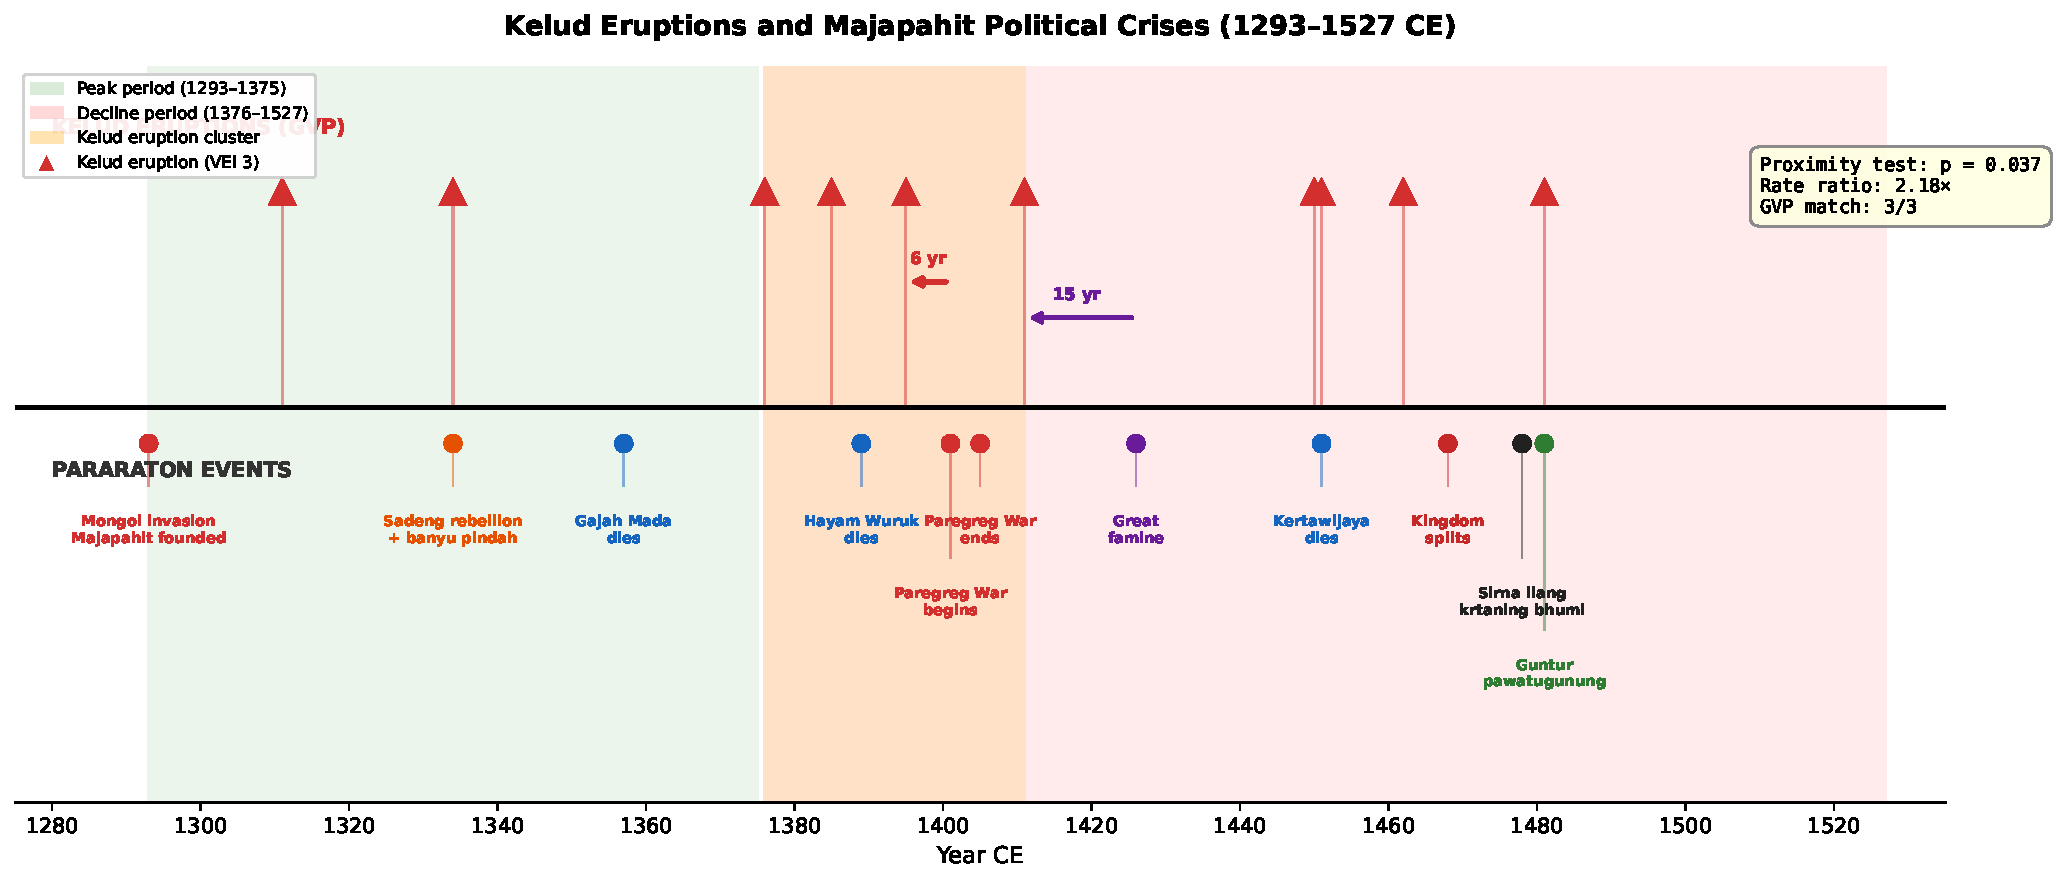
\includegraphics[width=\textwidth]{figures/fig1_timeline.pdf}
\caption{Timeline of Kelud eruptions (top) and Pararaton political events (bottom), 1293--1527~CE.
The shaded region marks the 1376--1411 eruption cluster.}
\label{fig:timeline}
\end{figure}

\subsection{Eruption rate}

During Majapahit's peak (83 years), Kelud erupted twice (2.4/century).
During the decline (152 years), it erupted eight times (5.3/century)---a rate ratio of 2.18 (Table~\ref{tab:rates}).
However, the Poisson exact test yields $p = 0.255$, indicating that this difference is not statistically significant given the small counts involved.

\begin{table}[htbp]
\centering
\caption{Kelud eruption frequency during Majapahit's peak and decline.}
\label{tab:rates}
\begin{tabular}{lcccc}
\toprule
Period & Duration & Eruptions & Rate (/century) & Poisson $p$ \\
\midrule
Peak (1293--1375)    & 83 yr  & 2 & 2.4 & \multirow{2}{*}{0.255} \\
Decline (1376--1527) & 152 yr & 8 & 5.3 & \\
\midrule
\multicolumn{3}{l}{Rate ratio (decline/peak)} & \textbf{2.18} & \\
\bottomrule
\end{tabular}
\end{table}

\subsection{Pararaton--GVP match}

All three Pararaton geological events match the GVP record: \textit{banyu pindah} (1334 = Kelud 1334, exact), \textit{pagunung anyar} (1374 $\approx$ Kelud 1376, $\Delta = 2$~yr), and \textit{guntur pawatugunung} (1481 = Kelud 1481, exact).
The \textit{pagunung anyar} (`new mountain') may reference mud volcanism rather than Kelud itself, as the Brantas delta produces active mud volcanoes to the present day---most dramatically the LUSI (Lumpur Sidoarjo) eruption active since 2006 \citep{davies2011,satyana2015}.

\subsection{Multiple testing correction}

Table~\ref{tab:correction} presents all $p$-values with Bonferroni and Holm-Bonferroni corrections.

\begin{table}[htbp]
\centering
\caption{Multiple testing correction. No test survives either correction at $\alpha = 0.05$.}
\label{tab:correction}
\begin{tabular}{lccl}
\toprule
Test & $p$ (uncorr.) & $p$ (Holm adj.) & Verdict \\
\midrule
Proximity permutation   & 0.037 & 0.222 & n.s.\ after correction \\
Post-eruption window 5yr  & 0.118 & 0.588 & n.s. \\
Post-eruption window 10yr & 0.214 & 0.855 & n.s. \\
Post-eruption window 15yr & 0.456 & 0.456 & n.s. \\
Post-eruption window 20yr & 0.445 & 0.890 & n.s. \\
Poisson rate test       & 0.255 & 0.764 & n.s. \\
\bottomrule
\end{tabular}
\end{table}

\noindent
The proximity permutation test ($p = 0.037$) is the only test significant at the uncorrected $\alpha = 0.05$ level, but does not survive Bonferroni ($\alpha_\mathrm{adj} = 0.0083$) or Holm-Bonferroni correction.
If the proximity test were pre-registered as the sole primary analysis, it would remain significant without correction; however, as we report six tests, correction is appropriate.

\section{Discussion}

\subsection{Convergence despite non-significance}

While no individual test provides definitive statistical evidence after correction, the three independent lines of evidence---temporal proximity, rate asymmetry, and textual cross-reference---converge in the same direction.
The 3/3 Pararaton--GVP match cannot be expressed as a $p$-value but represents a qualitative confirmation that the chronicle's geological awareness is empirically grounded.

We tentatively propose a Volcanic Mandala Model: Kelud eruptions disrupted the agricultural surplus of the Brantas basin, weakening the mandala centre's capacity to manage factional tensions.
The 1376--1411 eruption cluster (four eruptions in 35 years) coincides with the Paregreg Civil War and the onset of mandala contraction.
This model does not replace conventional explanations (succession, Islam, trade) but adds an environmental trigger that may explain their convergent timing.

\subsection{Limitations}

The sample size is small (10 eruptions, 18 crises), limiting statistical power.
GVP dates for pre-instrumental eruptions are approximate.
The Pararaton's chronology is debated \citep{noorduyn1978}.
Most critically, temporal correlation does not establish causation; the proposed agricultural-disruption mechanism requires archaeological confirmation via stratigraphic evidence at Trowulan.

The post-eruption window tests are non-significant, suggesting that eruption--crisis association is a population-level pattern rather than a sharp threshold effect---consistent with volcanic stress acting as chronic destabiliser rather than acute trigger.

\subsection{The Pararaton as geological document}

The chronicle's editorial structure suggests awareness of volcanic causation: it records geological events (unusual for Southeast Asian royal chronicles), and its final entry is an eruption, not a political event.
The \textit{candrasengkala} `Sirna ilang krtaning bhumi' (1478) is conventionally translated `vanished, lost, the glory of the earth', but can also be read `vanished, lost---by the action of the earth' \citep{satyana2015}.

\section{Conclusion}

This exploratory analysis finds suggestive but not statistically definitive evidence that Kelud eruptions temporally preceded Majapahit political crises.
The proximity test ($p = 0.037$) does not survive correction for multiple comparisons.
However, the convergence of temporal proximity, eruption rate asymmetry, and independent GVP confirmation of all three Pararaton geological events generates a hypothesis that warrants testing with larger datasets and archaeological evidence.

The Pararaton author's decision to end the chronicle with \textit{guntur pawatugunung}---the mountain's thunder---may reflect genuine causal understanding of the relationship between volcanic activity and political collapse.
Whether this understanding is correct remains, for now, an open question.

\section*{AI disclosure}

Claude (Anthropic) was used for statistical analysis, multiple testing correction, and drafting assistance.
All hypotheses and interpretive claims are the author's own.

\section*{Data availability}

The GVP eruption database is available at \url{https://volcano.si.edu}.
Analysis scripts are available at \url{https://github.com/neimasilk/volcarch-repo}.

\bibliographystyle{apalike}

\begin{thebibliography}{99}

\bibitem[Brandes, 1896]{brandes1896}
Brandes, J.L.A. (1896).
\textit{Pararaton (Ken Arok) of het Boek der Koningen van Tumapel en van Majapahit}.
Verhandelingen van het Bataviaasch Genootschap, 49.
Batavia: Albrecht \& Co.

\bibitem[Davies et al., 2011]{davies2011}
Davies, R.J., Brumm, M., Manga, M., et al. (2011).
The East Java mud volcano (2006 to present): An earthquake or drilling trigger?
\textit{Earth and Planetary Science Letters}, 272(3--4), 627--638.

\bibitem[Global Volcanism Program, 2024]{gvp2024}
Global Volcanism Program (2024).
\textit{Volcanoes of the World}, v.~5.2.8.
Smithsonian Institution.
\url{https://doi.org/10.5479/si.GVP.VOTW5-2024.5.2}

\bibitem[Noorduyn, 1978]{noorduyn1978}
Noorduyn, J. (1978).
Majapahit in the fifteenth century.
\textit{Bijdragen tot de Taal-, Land- en Volkenkunde}, 134(2/3), 207--274.

\bibitem[Pigeaud, 1960--1963]{pigeaud1967}
Pigeaud, T.G.T. (1960--1963).
\textit{Java in the 14th Century: A Study in Cultural History}, 5 vols.
The Hague: Martinus Nijhoff.

\bibitem[Reid, 1993]{reid1993}
Reid, A. (1993).
\textit{Southeast Asia in the Age of Commerce, 1450--1680}.
New Haven: Yale University Press.

\bibitem[Ricklefs, 2001]{ricklefs2001}
Ricklefs, M.C. (2001).
\textit{A History of Modern Indonesia since c.~1200}, 3rd ed.
Basingstoke: Palgrave.

\bibitem[Satyana, 2015]{satyana2015}
Satyana, A.H. (2015).
Gunung lumpur, bencana geologi, dan mitos: Sebuah review dan kajian Sidoarjo.
\textit{Academia.edu preprint}.

\bibitem[Wolters, 1982]{wolters1982}
Wolters, O.W. (1982).
\textit{History, Culture, and Region in Southeast Asian Perspectives}.
Singapore: Institute of Southeast Asian Studies.

\end{thebibliography}

\end{document}
